\newcommand{\formalcontexttable}{%
\begin{table}[]
\centering
\caption{Formal context}
\label{tab:formal_context}
\begin{tabular}{|l|c|c|c|c|c|}
\hline
          & $x_A$           & $x_B$           & $x_C$           & $x_D$           & \dots \\ \hline
$c_1$         & $\times$    & $\times$    &             &             &        \\ \hline
$c_2$         &             &             & $\times$    & $\times$    &        \\ \hline
$c_1 \vee c_2$ & $\times$    & $\times$    & $\times$    & $\times$    &        \\ \hline
$\vdots$      &             &             &             &             & $\ddots$ \\ \hline
\end{tabular}%
\end{table}%
}

\newcommand{\dendogram}{%
\begin{figure}[]
\centering
\caption{Dendrogram with objects on the bottom.}
\label{fig:dendrogram}

\begin{tikzpicture}[scale=1]
% Positions of objects (bottom)
\node (A) at (0,0) {$x_A$};
\node (B) at (2,0) {$x_B$};
\node (C) at (4,0) {$x_C$};
\node (D) at (6,0) {$x_D$};

% Merge A and B
\coordinate (ABtop) at (1,1);
\draw (A) -- (0,1) -- (ABtop) -- (2,1) -- (B);

% Merge C and D
\coordinate (CDtop) at (5,1);
\draw (C) -- (4,1) -- (CDtop) -- (6,1) -- (D);

% Merge AB and CD
\coordinate (root) at (3,2);
\draw (ABtop) --(1,2) -- (5,2) -- (CDtop);

\end{tikzpicture}
\end{figure}
}

\newcommand{\lattice}{%
\begin{figure}[h]
\centering
\caption{Concept lattice for the transposed formal context.}
\label{fig:concept_lattice}

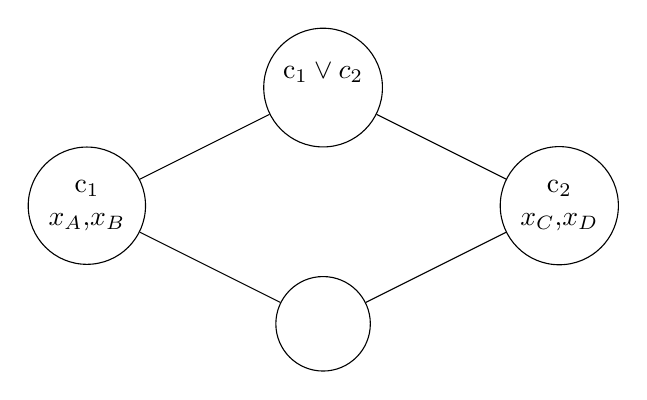
\begin{tikzpicture}[scale=1, every node/.style={draw, circle, align=center, minimum width=1.2cm, minimum height=1.2cm}]
% Nodes
\node (top) at (0,3) {c$_1 \vee c_2$ \\ };
\node (left) at (-3,1.5) {c$_1$ \\ $x_A$,$x_B$};
\node (right) at (3,1.5) {c$_2$ \\ $x_C$,$x_D$};
\node (bottom) at (0,0) {};

% Edges
\draw (top) -- (left);
\draw (top) -- (right);
\draw (left) -- (bottom);
\draw (right) -- (bottom);

\end{tikzpicture}
\end{figure}
}
